\section{Performance Assessment}
%

The performance of the proposed method is assessed by comparing its results to those of a state-of-the-art software package. Performance is measured quantitatively for canonical image masks defined by spheres of various radii and locations and qualitatively for a variety of examples from real MRI and CT scans. \\ \\
%
For the canonical cases, image masks are defined for each voxel ${v}$ by the following:
\begin{align} 
	v &=  \begin{cases}
		1, & \text{if}\ d \left(\bm{v_C},\bm{C}\right) \le R \\
		0, & \text{otherwise}
	\end{cases}
\end{align}
where $d$ is the Euclidean distance, $\bm{v_C}$ is the center of voxel $v$, $\bm{C}$ is the center of the spherical image mask, and $R$ is its radius. The background image is assumed to have a 256 $\times$ 256 $\times$ 256 voxel resolution. \\ \\
%
In order to quantify performance, two error metrics are defined: a shape error and a volume error. These errors are defined in conjunction with a corresponding ``perfect sphere''. Each b-rep from these examples has an associated perfect sphere we are approximating, against which the error mismatches are measured. These metrics have two sources of error, as described by Young \textit{et al.}~\cite{young_2008}: 1) the error of approximating the perfect sphere with a binary image mask, or the \textit{image-based error}, and 2) the error of attempting to reconstruct the binary image mask with a b-rep, or the method's ability to \textit{converge to geometry}. The image mask defined above of course does not yield perfect image-based accuracy, but for these purposes, we will assume that the image-based error is negligible and will focus on the ability of the method to converge to geometry.\\ \\
%
The shape error measures the surface deviation of the resultant b-rep from the perfect sphere it is meant to reconstruct. Each facet of the resulting b-rep is projected onto the underlying sphere. The normal of each facet is compared to the normal of the underlying sphere at the centroid of the projected facet by computing the magnitude of their cross product. A weighted sum is performed as a means to integrate over the area of the b-rep, and finally the sum is normalized by the surface area of the b-rep to provide a range of values from 0 to 1, inclusive. Thus, the shape error $e_s$ is defined as:
\begin{equation} 
	e_s = \frac{1}{A} \sum \limits_{f\in\mathcal{F}} \lVert {\bf n}_f \times {\bf n}_s \rVert
\end{equation}
where $A$ is the surface area of the b-rep, $f$ is a facet on the b-rep belonging to the set of all b-rep facets $\mathcal{F}$, ${\bm n}_f$ is the normal of facet $f$, and ${\bm n}_s$ is the normal of the associated sphere at the centroid of the projected facet $f$ onto the sphere. \\ \\
%
The volume error measures the unsigned difference in volumes enclosed by the b-rep and associated perfect sphere. If we define the surface of facet $f$ as $\gamma_f$,  ${\bm x} \in \gamma_f$, $r = \lVert {\bm x} \rVert$, $d\alpha$ as an area element on the sphere of the projected b-rep facet, and $R$ as the radius of the underlying perfect sphere, we define a normalized volume error $e_v$ as:
\begin{equation}
	e_v = \frac{1}{4\pi R^2} \Big[\sum \limits_{f \in \mathcal{F}\textsl{}} \ \int \limits_{\gamma_f} (r - R)^2 d\alpha \Big]^{1/2}
\end{equation}
Each b-rep facet is projected onto the underlying perfect sphere. Integrals are performed numerically on the projected facet. Six quadrature points were found to provide sufficent accuracy. Finally, the quantity is made dimensionless by normalizing by the surface area of the underlying perfect sphere.
\\ \\
%
The shape and volume errors are compared between the commercial software and the proposed method for the canonical sphere case while independently varying three parameters: 1) final b-rep resolution, 2) sphere radius, and 3) sphere center location. The purpose of these comparions is to show that the  method performs comparably to an established option, rather than specifically pointing to the supreriority of one method over the other. Optimal results were obtained from the commercial package by selecting the ``binarise before smoothing" option and performing 100 iterations of smart mask smoothing; standard options were chosen otherwise. \\ \\
%
\figref{graph1} shows the shape and volume errors for the two methods as the b-rep resolution is varied for a spherical mask centered in the image with a radius $R = 80$ voxels. See~\figref{demos1} for a visual comparison of the image mask and representative b-reps from the commercial code and proposed method. Default parameters were used in the commercial code for b-reps with $n \ge 2587$ vertices. For resolutions coarser than that, the ``target maximum error" was increased to allow results with $n < 2587$. When comparing the shape error of the two approaches, the proposed method performs at least as well as the commercial option for coarse meshes ($n < 2500$), and performs measurably better for finer b-reps ($n > 5000$). For the volume error, the proposed method performs better for b-reps with resolution less than ~5000 vertices, and asymptotes to a comparable value toward which the commercial software converges.\\ \\
\begin{figure}[ht!]
	\centering
	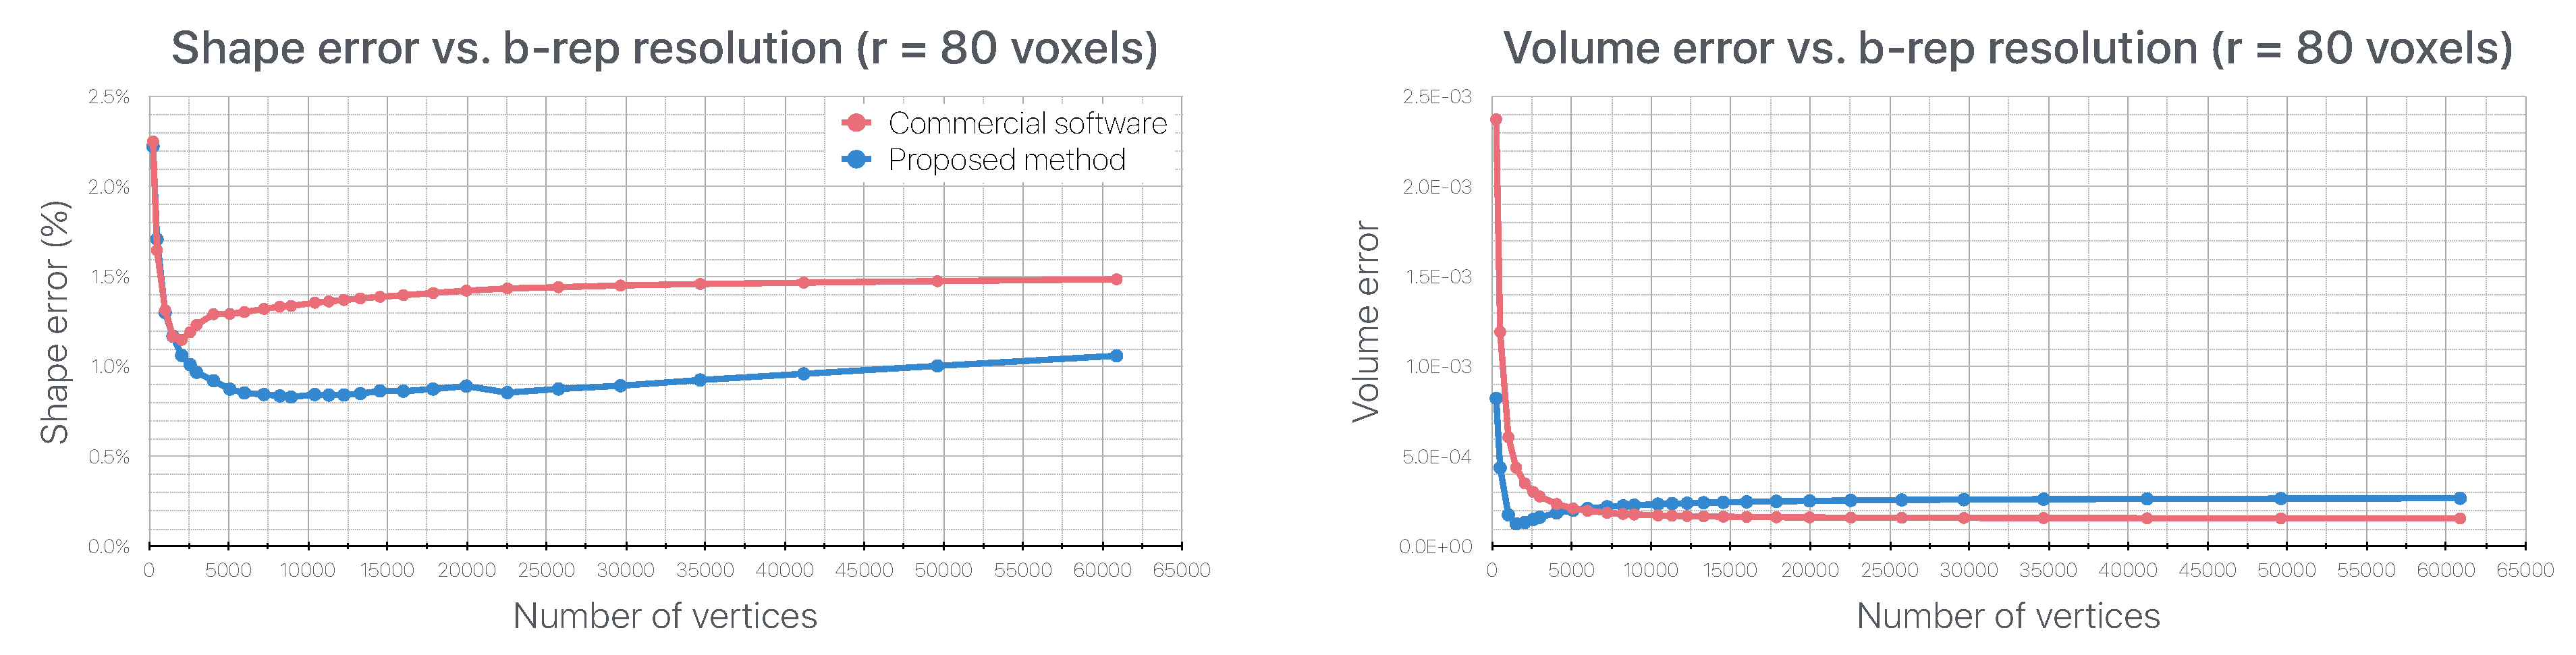
\includegraphics[scale=0.25]{media/7-performance/1-graph-1.pdf}
	\caption{Comparison of shape error (left) and volume error (right) between commercial software and proposed method as b-rep resolution is varied.}
	\label{fig:graph1}
\end{figure}
\begin{figure}[ht!]
	\centering
	\includegraphics[scale=0.25]{media/7-performance/3-demos-4.pdf}
	\caption{Image masks (green) and corresponding b-reps for commercial software (red) and proposed method (blue) for selected b-rep resolutions.}
	\label{fig:demos1}
\end{figure}
%
\figref{graph2} shows the error metrics when the radius of the spherical image mask if varied from 40 to 120 voxels, while keeping the sphere center fixed at the center of the image and the final b-rep resolution fixed at $n = 10428$ vertices. See~\figref{demos2} for representative examples of the image mask and resulting b-reps from the two methods. The sphere radius can be interpreted as an inverse measure of the curvature of the image mask. Larger radii correspond to smoother surfaces, whereas smaller radii correspond to regions where surfaces are changing rapidly. Both the shape and volume errors of the proposed method converge at roughly double the rate of the commercial approach's errors, albeit with larger coefficients in both cases. As expected, the proposed algorithm performs best for slowly-changing surfaces.
\begin{figure}[ht!]
	\centering
	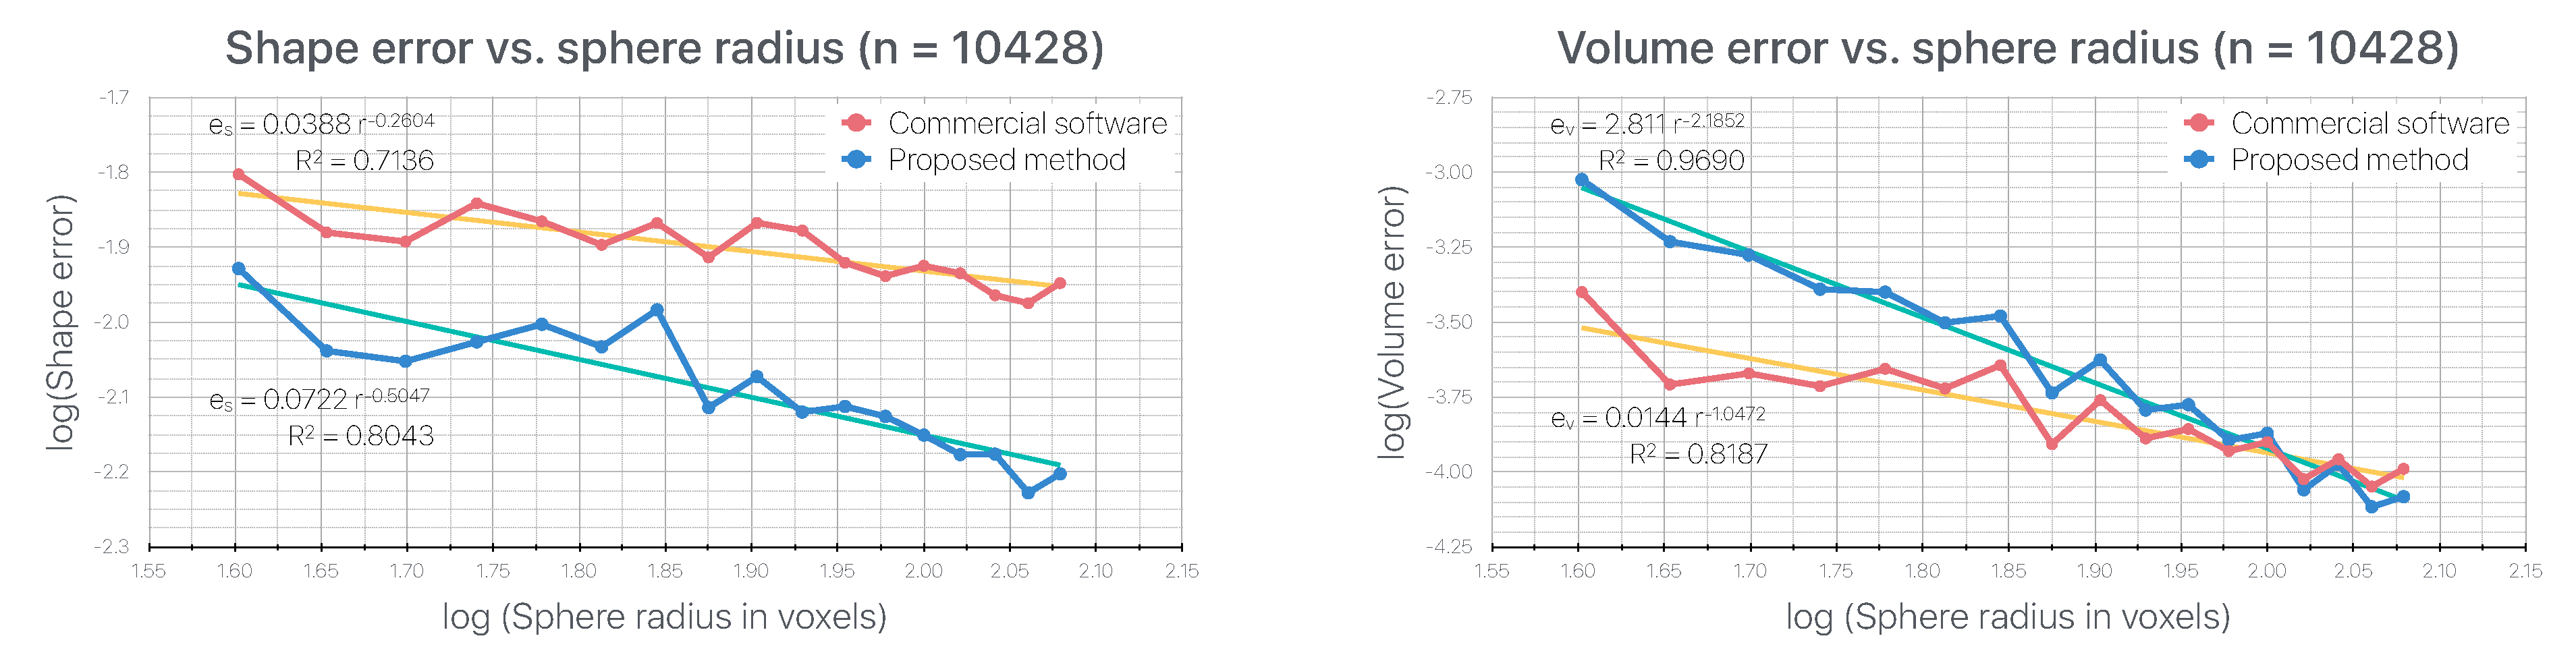
\includegraphics[scale=0.25]{media/7-performance/1-graph-2.pdf}
	\caption{Comparison of shape error (left) and volume error (right) between commercial software and proposed method as radius of sphere in image mask is varied.}
	\label{fig:graph2}
\end{figure}
\begin{figure}[ht!]
	\centering
	\includegraphics[scale=0.25]{media/7-performance/3-demos-5.pdf}
	\caption{Image masks (green) and corresponding b-reps for commercial software (red) and proposed method (blue) for selected sphere radii.}
	\label{fig:demos2}
\end{figure} \\ \\ 
%
Finally, the two methods are compared when a sphere of $R = 80$ voxels is translated along a unit direction defined by the vector $\bm{i}  + 2\bm{j} + 3\bm{k}$, while keeping the resulting b-rep fixed at $n = 10428$ vertices. The intent of this variation to test the sensitivity of the methods to the location of the object within the image itself. The b-reps should be consistently accurate regardless of where the object is located; indeed both methods show very low sensitivity to the translation of the object within the image, as shown in~\figref{graph3}. \\ \\
\begin{figure}[ht!]
	\centering
	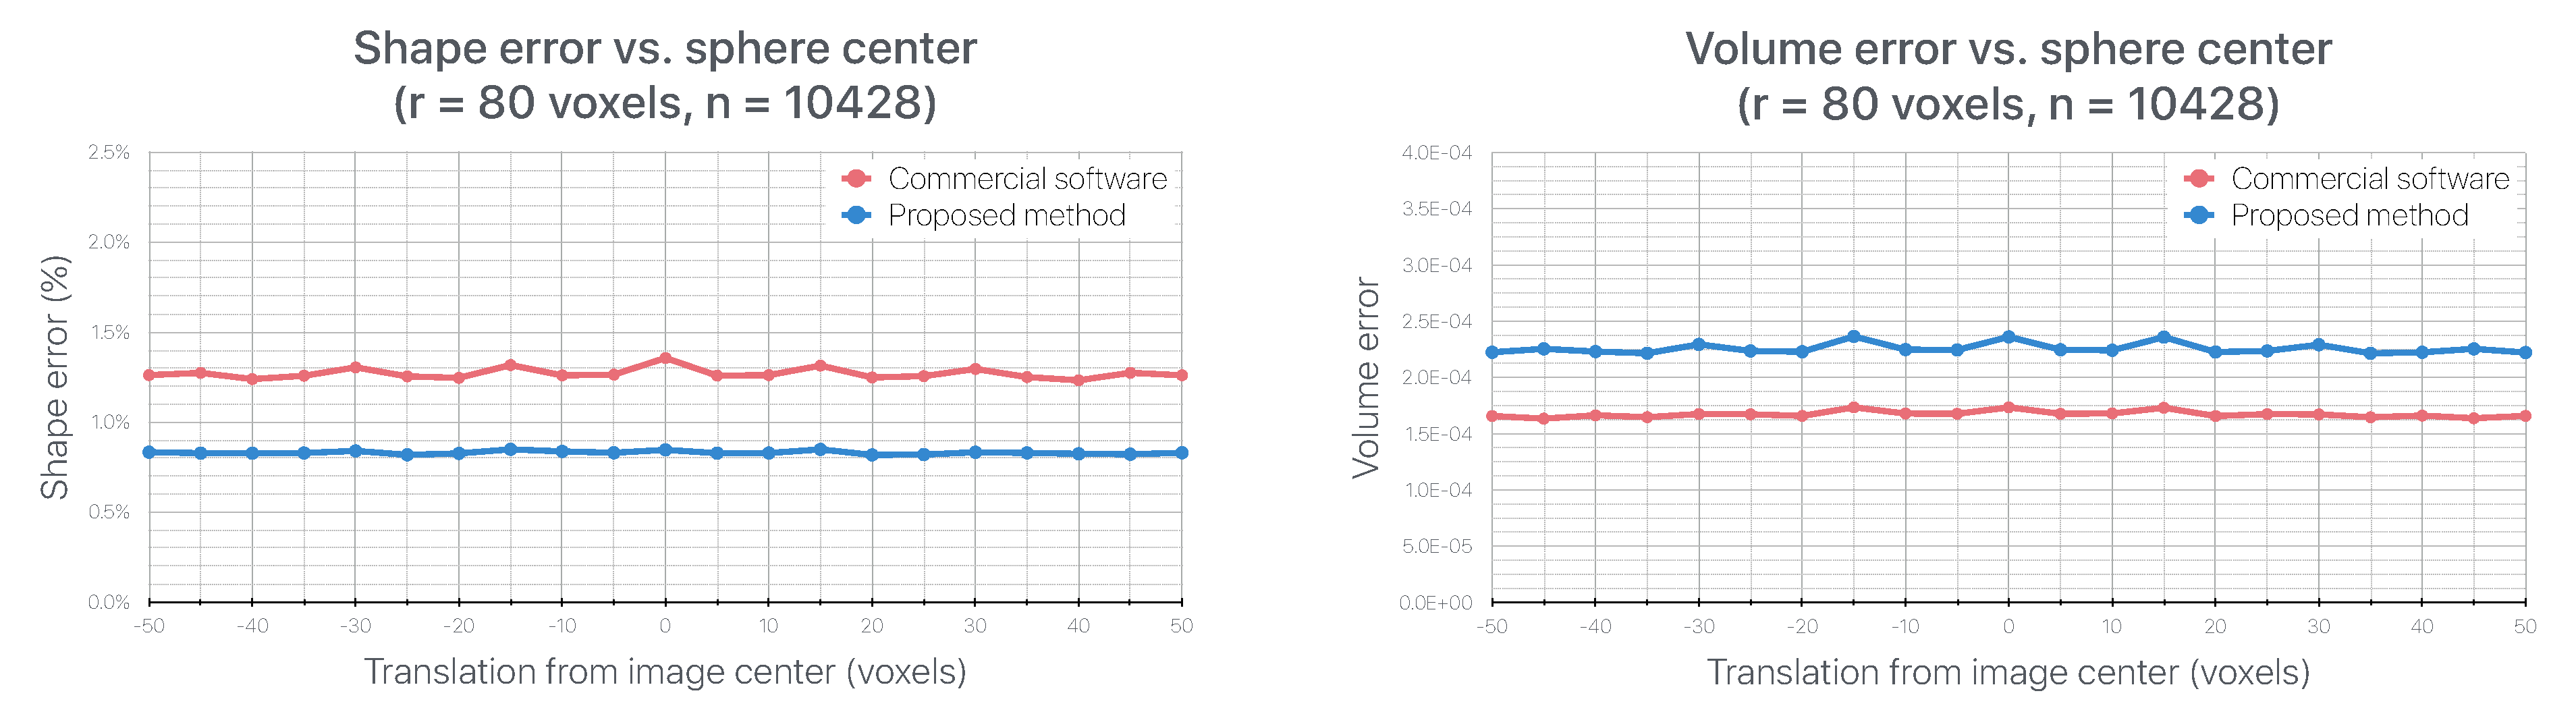
\includegraphics[scale=0.25]{media/7-performance/2-graph-3.pdf}
	\caption{Comparison of shape error (left) and volume error (right) between commercial software and proposed method as center of sphere in image mask is translated.}
	\label{fig:graph3}
\end{figure}
%
Qualitative comparisons are made for a number of real image examples. Images were segmented in Seg3D~\cite{Seg3D}. The resulting binary image masks were used as input to the two methods. B-rep resolutions were matched between the two approaches in all cases. See~\figref{example-meshes} for a comparison of image mask and resulting b-reps for a suite of examples. The proposed method perfoms comparably to the commercial approach in all cases, performing slighly better at smoothing surfaces and not quite as well for regions with high curvature. All examples completed for the proposed method on a 16 GB RAM laptop in less than 5 minutes.
\begin{figure}[ht!]
	\centering
	\includegraphics[scale=0.75]{media/7-performance/4-examples.pdf}
	\caption{Image masks (green) and corresponding b-reps for commercial software (red) and proposed method (blue) for various examples from MRI and CT. From top to botttom: brain~\cite{marcus_2007}, heart~\cite{winslow_2012}, lungs~\cite{rikxoort_2009}, distal femur~\cite{epperson_2013}, skull~\cite{clark_2013}, L5 lumbar~\cite{yao_2016}, pelvis~\cite{clark_2013}, upper left second molar (author's), liver~\cite{bilic_2019}, and example image with disjoint objects in image mask.}
	\label{fig:example-meshes}
\end{figure}